%\begin{figure*}[!h]
\begin{subfigure}{0.20\linewidth}
\centering
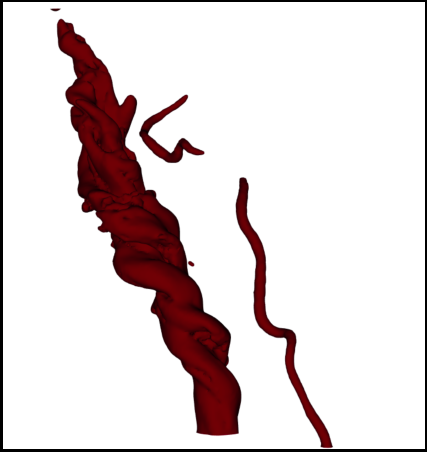
\includegraphics[width=0.9\linewidth]{Images/Tornado/zls.pdf}
\vspace{-1mm}
\caption{$ZLS_{T}$}
\label{fig:tornado_zls}
\end{subfigure}
\begin{subfigure}{0.20\linewidth}
\centering
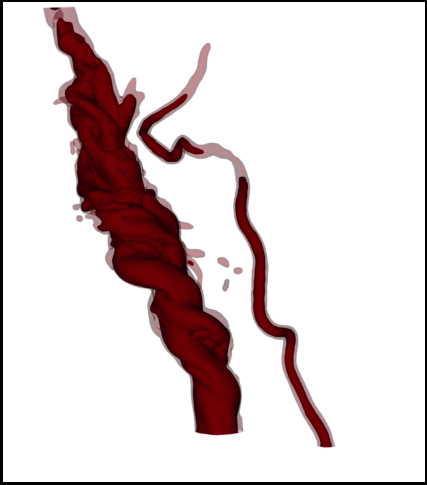
\includegraphics[width=0.9\linewidth]{Images/Tornado/fcls_50.pdf}
\vspace{-1mm}
\caption{+ $FCLS_{T,50\%}$}
\label{fig:tornado_fls}
\end{subfigure}
\begin{subfigure}{0.20\linewidth}
\centering
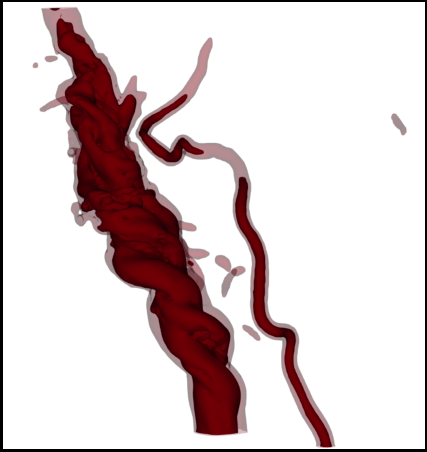
\includegraphics[width=0.9\linewidth]{Images/Tornado/fcls_68.pdf}
\vspace{-1mm}
\caption{+ $FCLS_{T,68\%}$}
\label{fig:tornado_fls}
\end{subfigure}
\begin{subfigure}{0.20\linewidth}
\centering
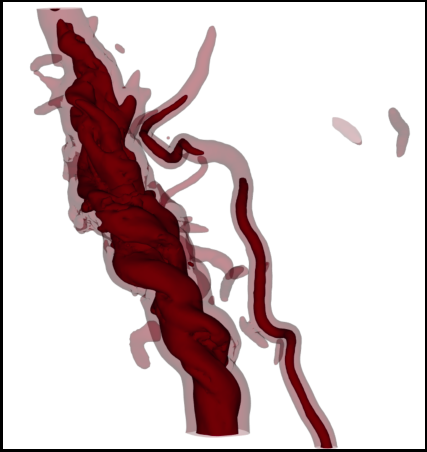
\includegraphics[width=0.9\linewidth]{Images/Tornado/fcls_95.pdf}
\vspace{-1mm}
\caption{+ $FCLS_{T,95\%}$}
\label{fig:tornado_fcls}
\end{subfigure}
\hfill
\begin{subfigure}{0.17\linewidth}
\centering
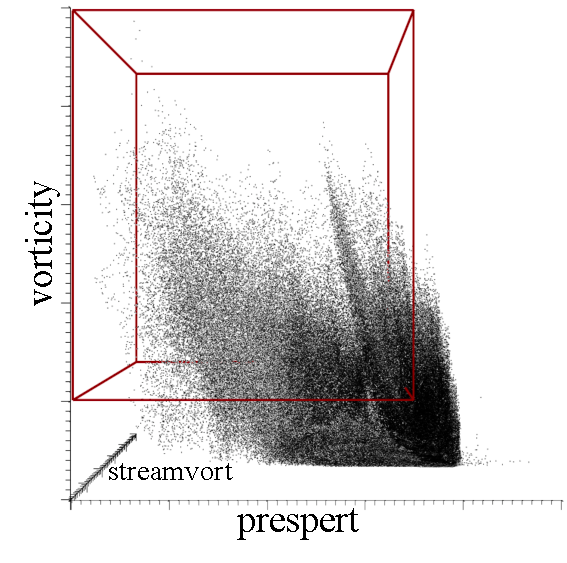
\includegraphics[width=\linewidth]{Images/Tornado/scatterplot3d.pdf}
\vspace{-4mm}
\caption{3D scatterplot of $\mathcal{A}$ and $T$ (red cuboid).} 
\label{fig:tornado_scatterplot}
\end{subfigure}
%\vspace{-2mm}
\caption{Visualization of EF-5 tornado vortices using vorticity, prespert and streamvort attributes. As in Figure~\ref{fig:tangle}, $FCLS_{T,C}$ formed wider envelopes as $C$ increased. Importantly, $FCLS_{T,C}$ visualized vortical structures of interest in the vicinity of the primary tornado vortex.}
%\vspace{-1mm}
\label{fig:tornado}
\end{figure*}

\begin{figure*}[h]
\begin{subfigure}{0.18\linewidth}
\centering
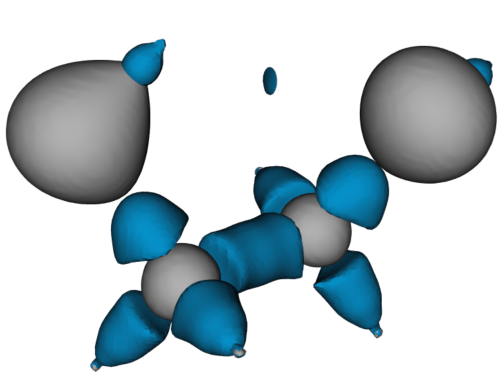
\includegraphics[width=\linewidth]{Images/EthaneDiol/gt.pdf}
\caption{$Rho_{isoval}=1.57$ (gray),\\ $s_{isoval}=-0.575$ (light blue)}
\label{}
\end{subfigure}
\begin{subfigure}{0.18\linewidth}
\centering
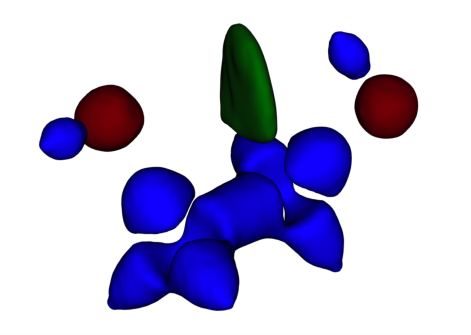
\includegraphics[width=\linewidth]{Images/EthaneDiol/zls_3.pdf}
\caption{$ZLS_{T}$}
\label{}
\end{subfigure}
\begin{subfigure}{0.18\linewidth}
\centering
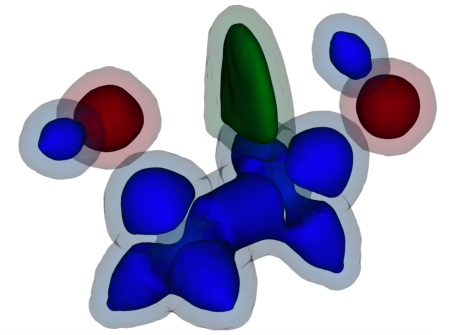
\includegraphics[width=\linewidth]{Images/EthaneDiol/fls_2_3.pdf}
\caption{$ZLS_{T}$ + $FLS_{T,2}$}
\label{}
\end{subfigure}
\begin{subfigure}{0.18\linewidth}
\centering
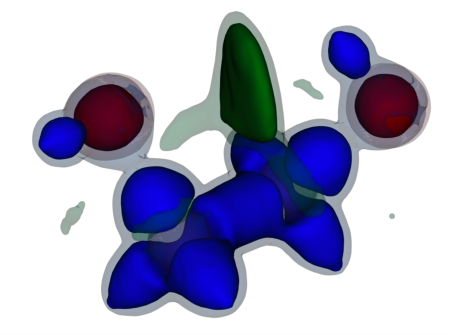
\includegraphics[width=\linewidth]{Images/EthaneDiol/fcls_68_3.pdf}
\caption{$ZLS_{T}$ + $FCLS_{T,68\%}$}
\label{}
\end{subfigure}
\begin{subfigure}{0.24\linewidth}
\centering
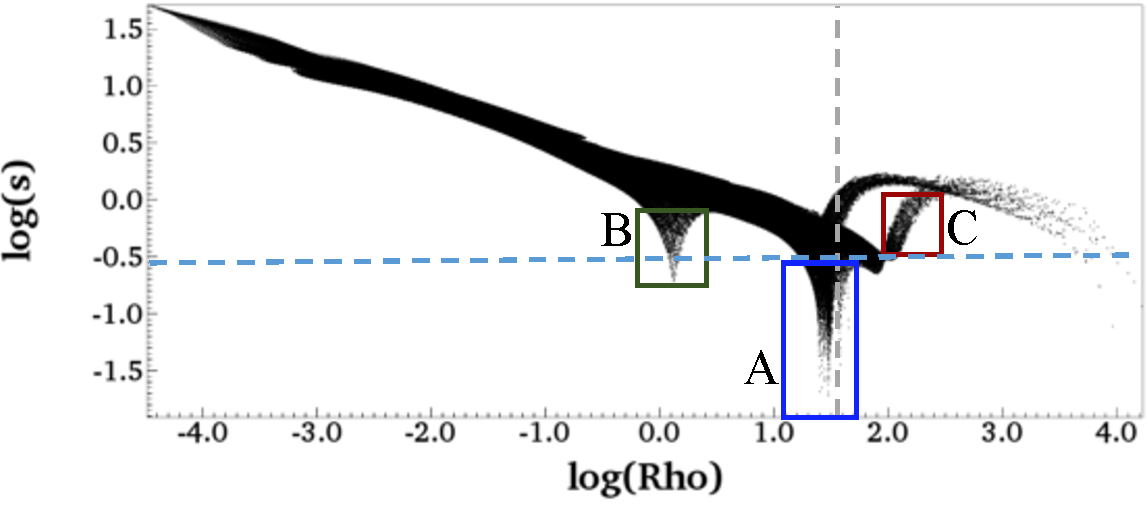
\includegraphics[width=\linewidth]{Images/EthaneDiol/scatterplot_3.pdf}
\caption{Attribute space 2D scatterplot, traits (labeled rectangular selections), and isovalues (dashed lines). We use $T = \left\{T_{A}, T_{B}, T_{C}\right\}$.} 
\label{}
\end{subfigure}
\caption{}
\label{}
\end{figure*}

\begin{figure*}[!h]
\begin{subfigure}{0.245\linewidth}
\centering
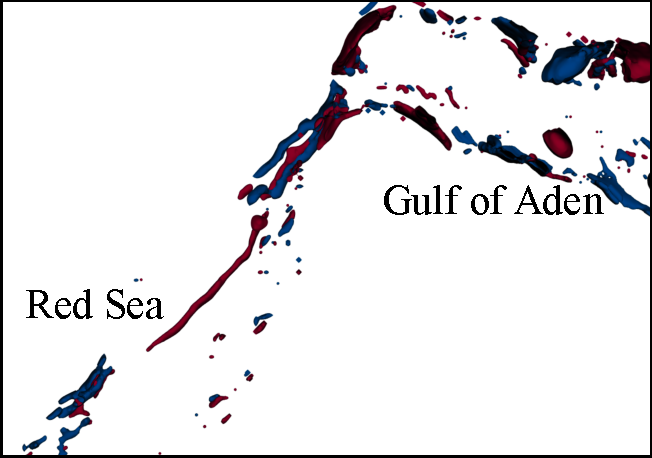
\includegraphics[width=\linewidth]{Images/RedSeaEddy/zls.pdf}
\vspace{-2mm}
\caption{$ZLS_{T}$}
\label{fig:rse_zls}
\end{subfigure}
\begin{subfigure}{0.245\linewidth}
\centering
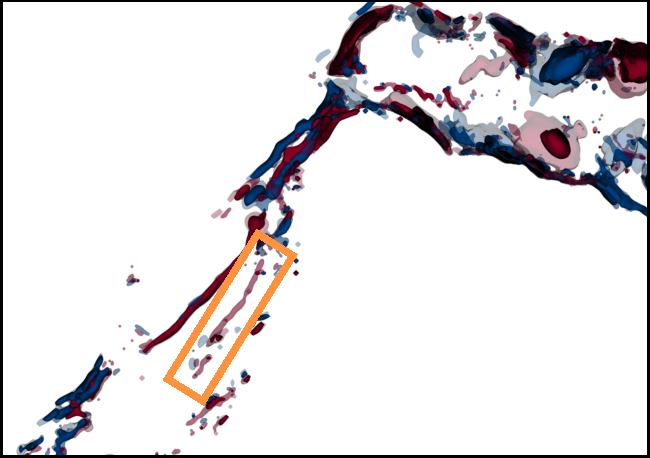
\includegraphics[width=\linewidth]{Images/RedSeaEddy/fcls_50.pdf}
\vspace{-2mm}
\caption{$ZLS_{T}$ + $FCLS_{T,50\%}$}
\label{fig:rse_fls}
\end{subfigure}
\begin{subfigure}{0.245\linewidth}
\centering
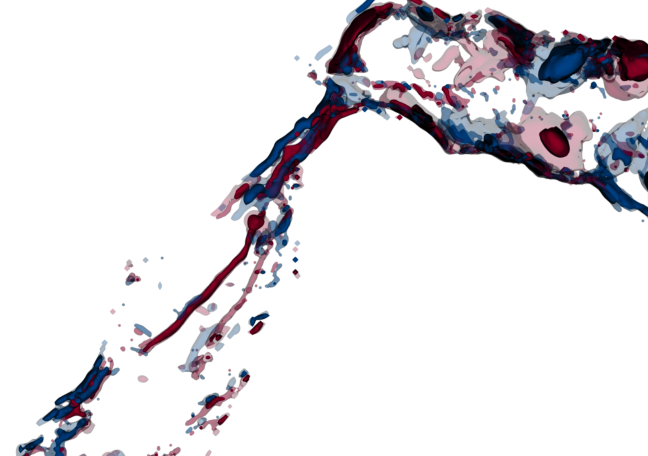
\includegraphics[width=\linewidth]{Images/RedSeaEddy/fcls_68.pdf}
\vspace{-2mm}
\caption{$ZLS_{T}$ + $FCLS_{T,68\%}$}
\label{fig:rse_fcls}
\end{subfigure}
\hfill
\begin{subfigure}{0.24\linewidth}
\centering
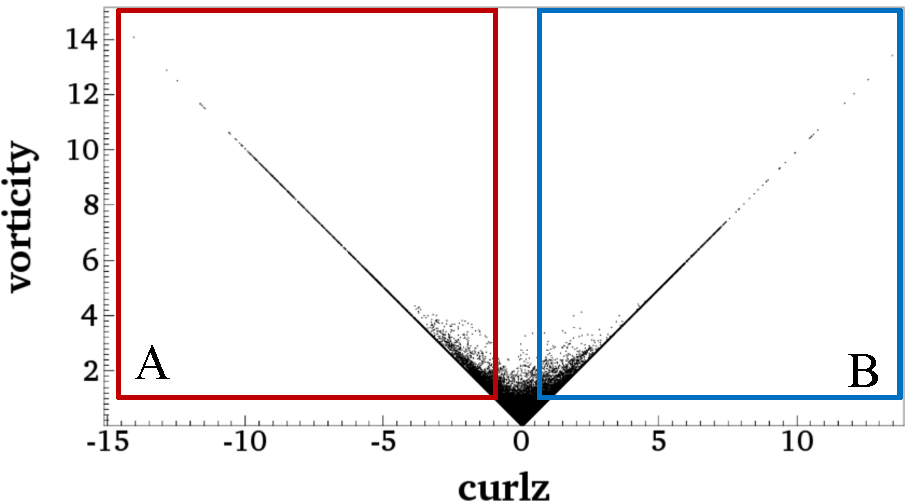
\includegraphics[width=0.95\linewidth]{Images/RedSeaEddy/scatterplot.pdf}
\vspace{-2mm}
\caption{Attribute space 2D scatterplot and traits (labeled rectangular selections). We use $T = \left\{T_{A}, T_{B}\right\}$.} 
\label{fig:rse_scatterplot}
\end{subfigure}
\vspace{-2mm}
\caption{Visualization of anticyclonic~($T_{A}$, red) and cyclonic~($T_{B}$, blue) eddies in the Gulf of Aden and part of the Red Sea using the derived attributes of vorticity magnitude and the z-component of curl. For this ensemble data set, $FCLS_{T,C}$ visualized additional paths and regions with eddies. The orange box in (c) highlights one such example.}
%\vspace{-1mm}
\label{fig:rse}
\end{figure*}

\begin{figure*}[!h]
\begin{subfigure}{0.2\linewidth}
\centering
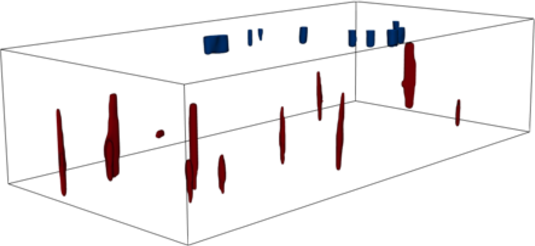
\includegraphics[width=\linewidth]{Images/Mantel/zls.pdf}
\vspace{-5mm}
\caption{$ZLS_{T}$}
\label{fig:mantel_zls}
\end{subfigure}
\begin{subfigure}{0.2\linewidth}
\centering
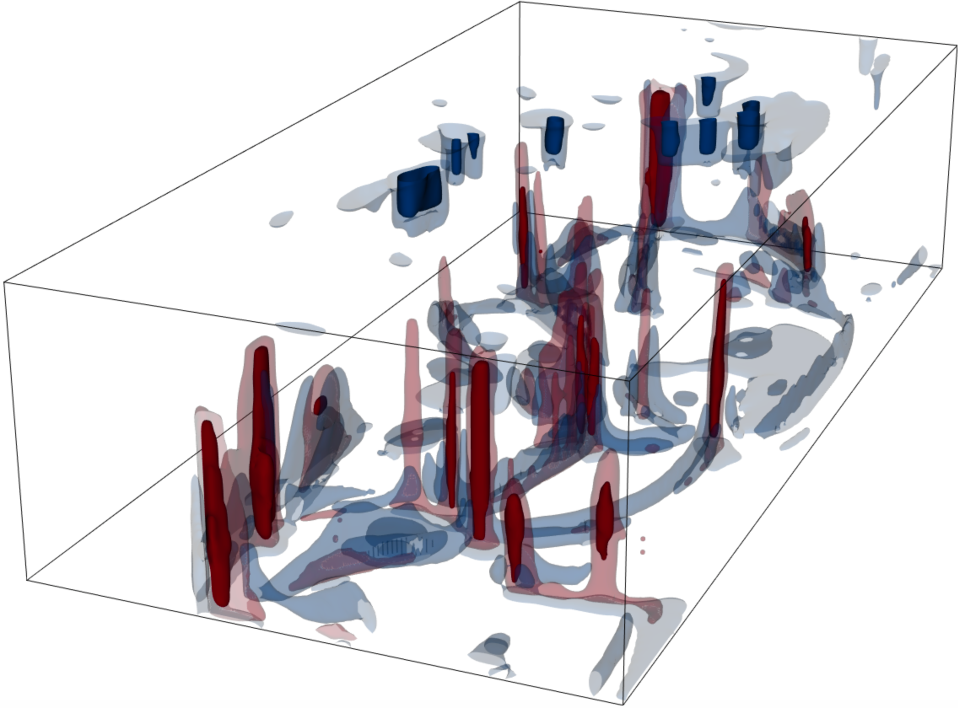
\includegraphics[width=\linewidth]{Images/Mantel/fcls_68.pdf}
\vspace{-5mm}
\caption{$ZLS_{T}$ + $FCLS_{T,68\%}$}
\label{fig:mantel_fls}
\end{subfigure}
\begin{subfigure}{0.295\linewidth}
\centering
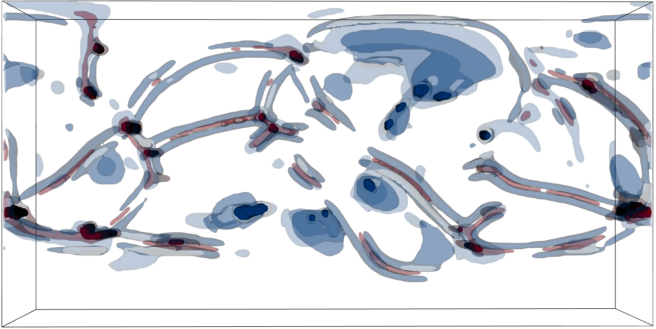
\includegraphics[width=0.9\linewidth]{Images/Mantel/fcls_68_v2.pdf}
\caption{$ZLS_{T}$ + $FCLS_{T,68\%}$}
\label{fig:mantel_fcls}
\end{subfigure}
\hfill
\begin{subfigure}{0.295\linewidth}
\centering
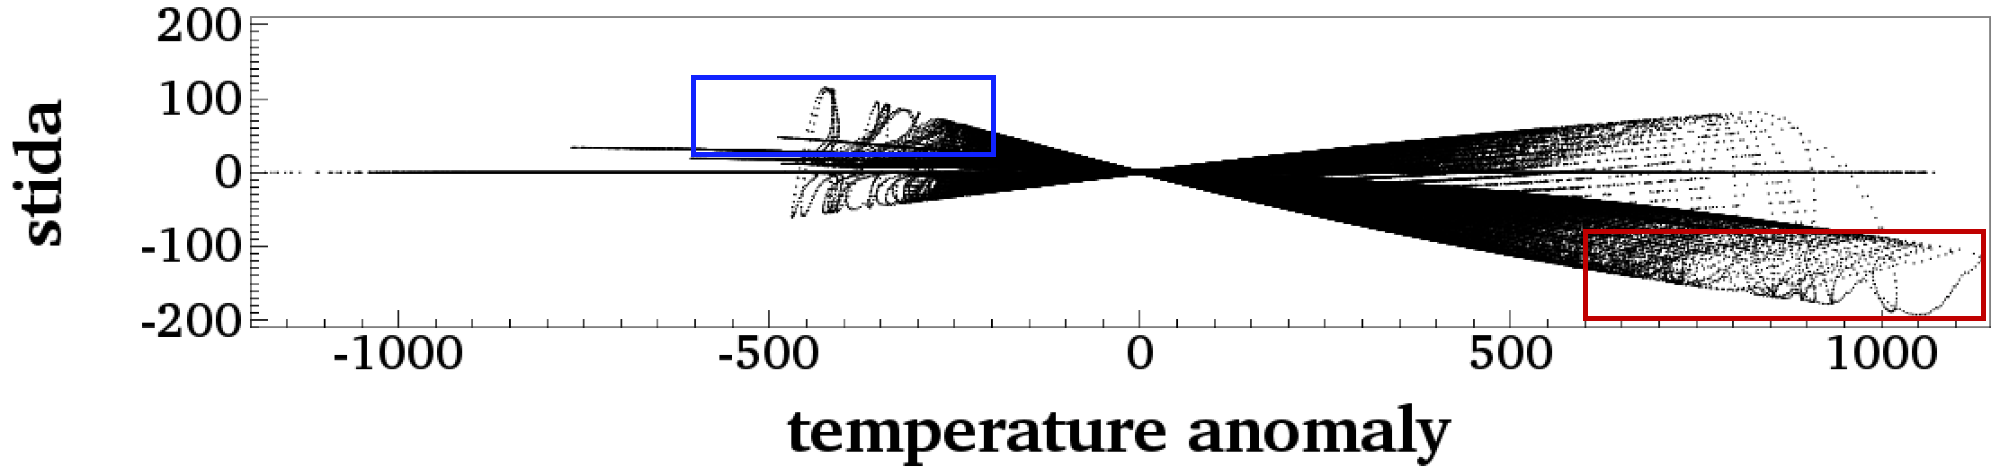
\includegraphics[width=\linewidth]{Images/Mantel/scatterplot.pdf}
%\vspace{-2mm}
\caption{Attribute space 2D scatterplot and traits (labeled rectangular selections). We use $T = \left\{T_{A}, T_{B}\right\}$.} 
\label{fig:mantel_scatterplot}
\end{subfigure}
\vspace{-2mm}
\caption{Visualization of rising hot plumes~($T_{A}$, red) and sinking material~($T_{B}$, blue) flow patterns in a subset of the spatial domain for the mantel data using the temperature anomaly and spin transition induced density anomaly~(stida) attributes.}
\label{fig:mantel}
\end{figure*}

%\begin{figure*}[!h]
\begin{subfigure}{0.195\linewidth}
\centering
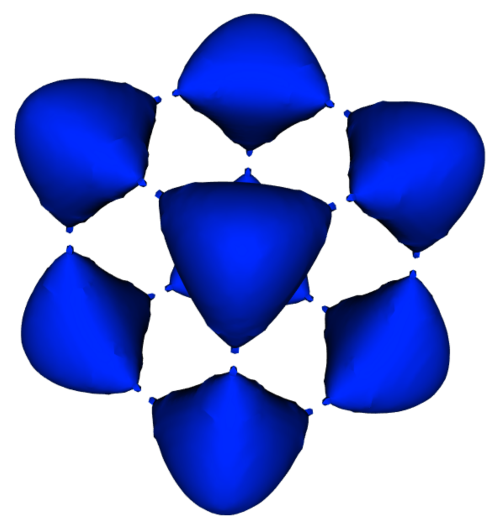
\includegraphics[width=0.8\linewidth]{Images/Tangle/gt.pdf}
\vspace{-2mm}
\caption{Ground truth, $isoval=62$}
\label{fig:tangle_gt}
\end{subfigure}
\begin{subfigure}{0.195\linewidth}
\centering
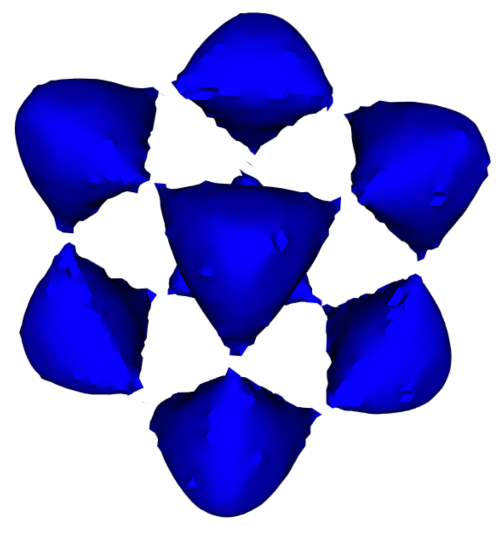
\includegraphics[width=0.8\linewidth]{Images/Tangle/zls.pdf}
\vspace{-2mm}
\caption{$ZLS_{T}$}
\label{fig:tangle_zls}
\end{subfigure}
\begin{subfigure}{0.195\linewidth}
\centering
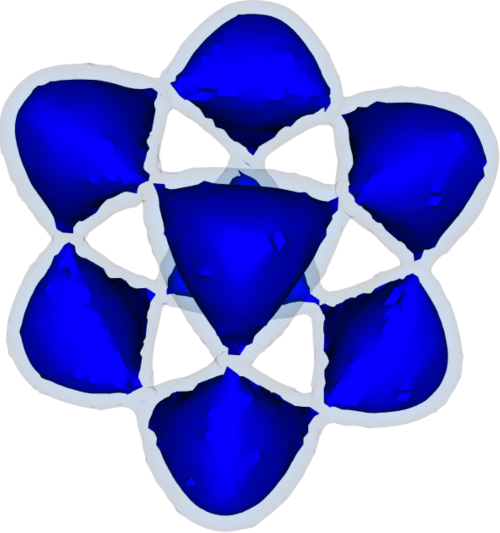
\includegraphics[width=0.8\linewidth]{Images/Tangle/fls.pdf}
\vspace{-2mm}
\caption{$ZLS_{T}$ + $FLS_{T,2}$}
\label{fig:tangle_fls}
\end{subfigure}
\begin{subfigure}{0.195\linewidth}
\centering
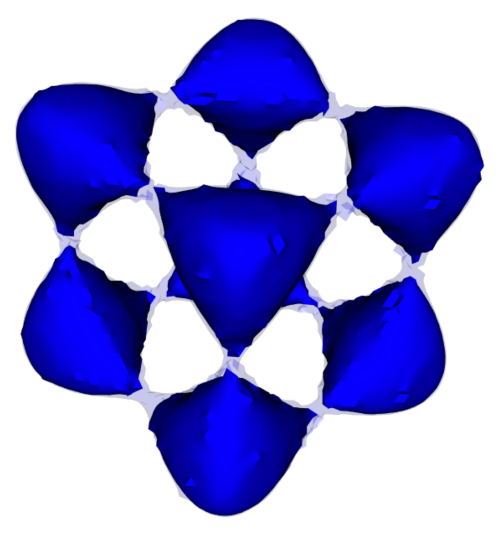
\includegraphics[width=0.8\linewidth]{Images/Tangle/fcls_68.pdf}
\vspace{-2mm}
\caption{$ZLS_{T}$ + $FCLS_{T,68\%}$}
\label{fig:tangle_fcls_68}
\end{subfigure}
\begin{subfigure}{0.195\linewidth}
\centering
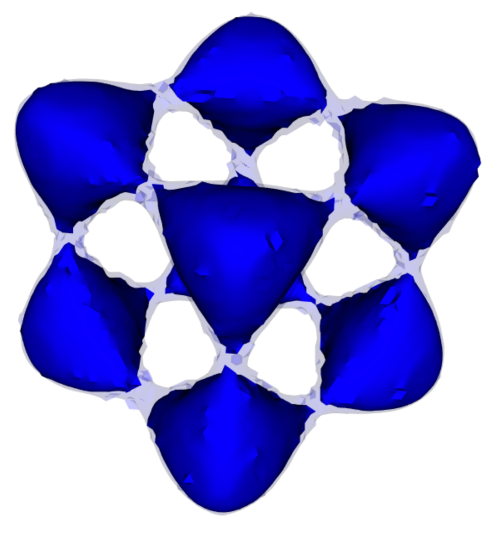
\includegraphics[width=0.8\linewidth]{Images/Tangle/fcls_95.pdf}
\vspace{-2mm}
\caption{$ZLS_{T}$ + $FCLS_{T,95\%}$}
\label{fig:tangle_fcls_95}
\end{subfigure}
\vspace{-2mm}
\caption{Visualization of sensitivity of the tangle function near values that form links between the multiple blobs. We use $T=[0,62]$.}
\vspace{-2mm}
\label{fig:tangle}
\end{figure*}

We demonstrated the use of feature confidence level-sets using five data sets.
%
Specifically, we considered an analytical tangle function~\cite{knoll2009fast}, an EF-5 Tornado~\cite{atmos10100578}, an ethanediol molecule from a chemistry simulation, Red Sea and Gulf of Aden~(RSGOA) eddy ensemble~\cite{sanikommu2020impact} and Earth's mantel convection~\cite{shahnas2017mid} data.
%
We defined between one to three traits per data set based on features of interest. 
%
%While our study demonstrated feature confidence level-sets for univariate and bivariate data, the approach can be applied to higher dimensions.\fix{Can we get an example in for a third?***}
%\fix{(Should we remove the part "the approach can be applied to higher dimensions" since we do not have results for n>2, but we can state the same in the future work section?)}.
%
In this study, each attribute was represented using a $mean$ and $SD$ field. 
%
For the RSGOA data set, we computed $mean$ and $SD$ fields from using 20 ensemble members. 
%
For other data sets, we synthetically estimated $SD$ for each scalar field of the multivariate data at each grid point by sampling the local neighborhood.
%
To evaluate our technique, we visualized the $ZLS_{T}$ both in isolation and augmented with $FCLS_{T,C}$. 
%
When visualized together, the $ZLS_{T}$ is shown using an opaque isosurface, and the $FCLS_{T,C}$ is shown using an isosurface colored with the same hue and 25\% opacity.
%
We used VisIt~\cite{childs2012visit} in our pipeline to render level-sets.

%also augment it with a semi-opaque, single feature level-set $FLS_{T,K}$ for some level $K$, or a feature confidence level-set $FCLS_{T,C}$ for some confidence $C$ (and level $\epsilon$).
%

%For all data sets considered, as expected we found $FLS_{T,K}$ has the shortcoming of discernibility.
%
%The $FLS_{T,K}$ level-set typically formed a ``shell'' like structure.
%
Across all data sets, the shape of $FCLS_{T,C}$ corresponded to the uncertainty of the data in the spatial domain.
%
For example, for the analytical tangle function where uncertainty is higher near the links between the blobs for the trait specified, we found comparing Figures~\ref{fig:tangle_fcls_68} and~\ref{fig:tangle_fcls_95} the $FCLS_{T,C}$ envelope expanded between the links in response to increasing the value of $C$, but not significantly on the exterior of the blob surface.
%
By leveraging the information pertaining to field distribution~($mean$, $SD$), $FCLS_{T,C}$ provided secondary structure visualization based on uncertainty.
%
%\fix{(Should we add boxes/zoomed-in views to the examples below to illustrate improvements achieved using our  $FCLS_{T,C}$? For example, we may show boxes where molecular topology is discovered nicely or one link and one blob in the case of the tangle function. This will enhance the interpretability of results.)}
%
For example, we observed the structure of weaker tornado vortices~(Figure~\ref{fig:tornado}), topological structure information for the ethanediol molecule~(Figure~\ref{fig:ethanediol}), regions with anticyclonic and cyclonic eddies across ensemble members~(Figure~\ref{fig:rse}), and the proximity as well as relationship of contrasting features in the spatial domain for the mantel data set~(Figure~\ref{fig:mantel_fcls_68_v2}).
%
%Importantly, for the traits selected, the secondary structures produced using $FCLS_{T,C}$ did not overlap one another.
%
%In contrast, for the same traits, $FLS_{T,K}$ resulted in overlapping and occluding level-sets~(see Figure~\ref{fig:rse_fls}).
%
%We provide supplementary visualizations and comparisons in the additional material. 
 
